\begin{frame}[t]{Diode}

    \textbf{Ziel - Darstellung von Bauteilkennlinie}
    
    \begin{spacing}{0.6} \begin{tiny}
    
    Eine Diode wird oft durch Ihre Durchlassspannung klassifiziert. Dies ist die Spannung ab der die Diode leitend wird. Leitend ist Sie, wenn ein Strom fließt. Dieses Verhalten möchten
    wir in einem kleinen simulativen Experiment herausarbeiten. 
    \end{tiny} \end{spacing}
    \begin{spacing}{0.9} \begin{tiny}
    \begin{table}[h!]
      \begin{tabular}{p{3cm} p{7cm}}
        \hline
        \textbf{Erstellung des Schaltplans} & \\
        \hline \\
        \begin{minipage}{.3\textwidth}
          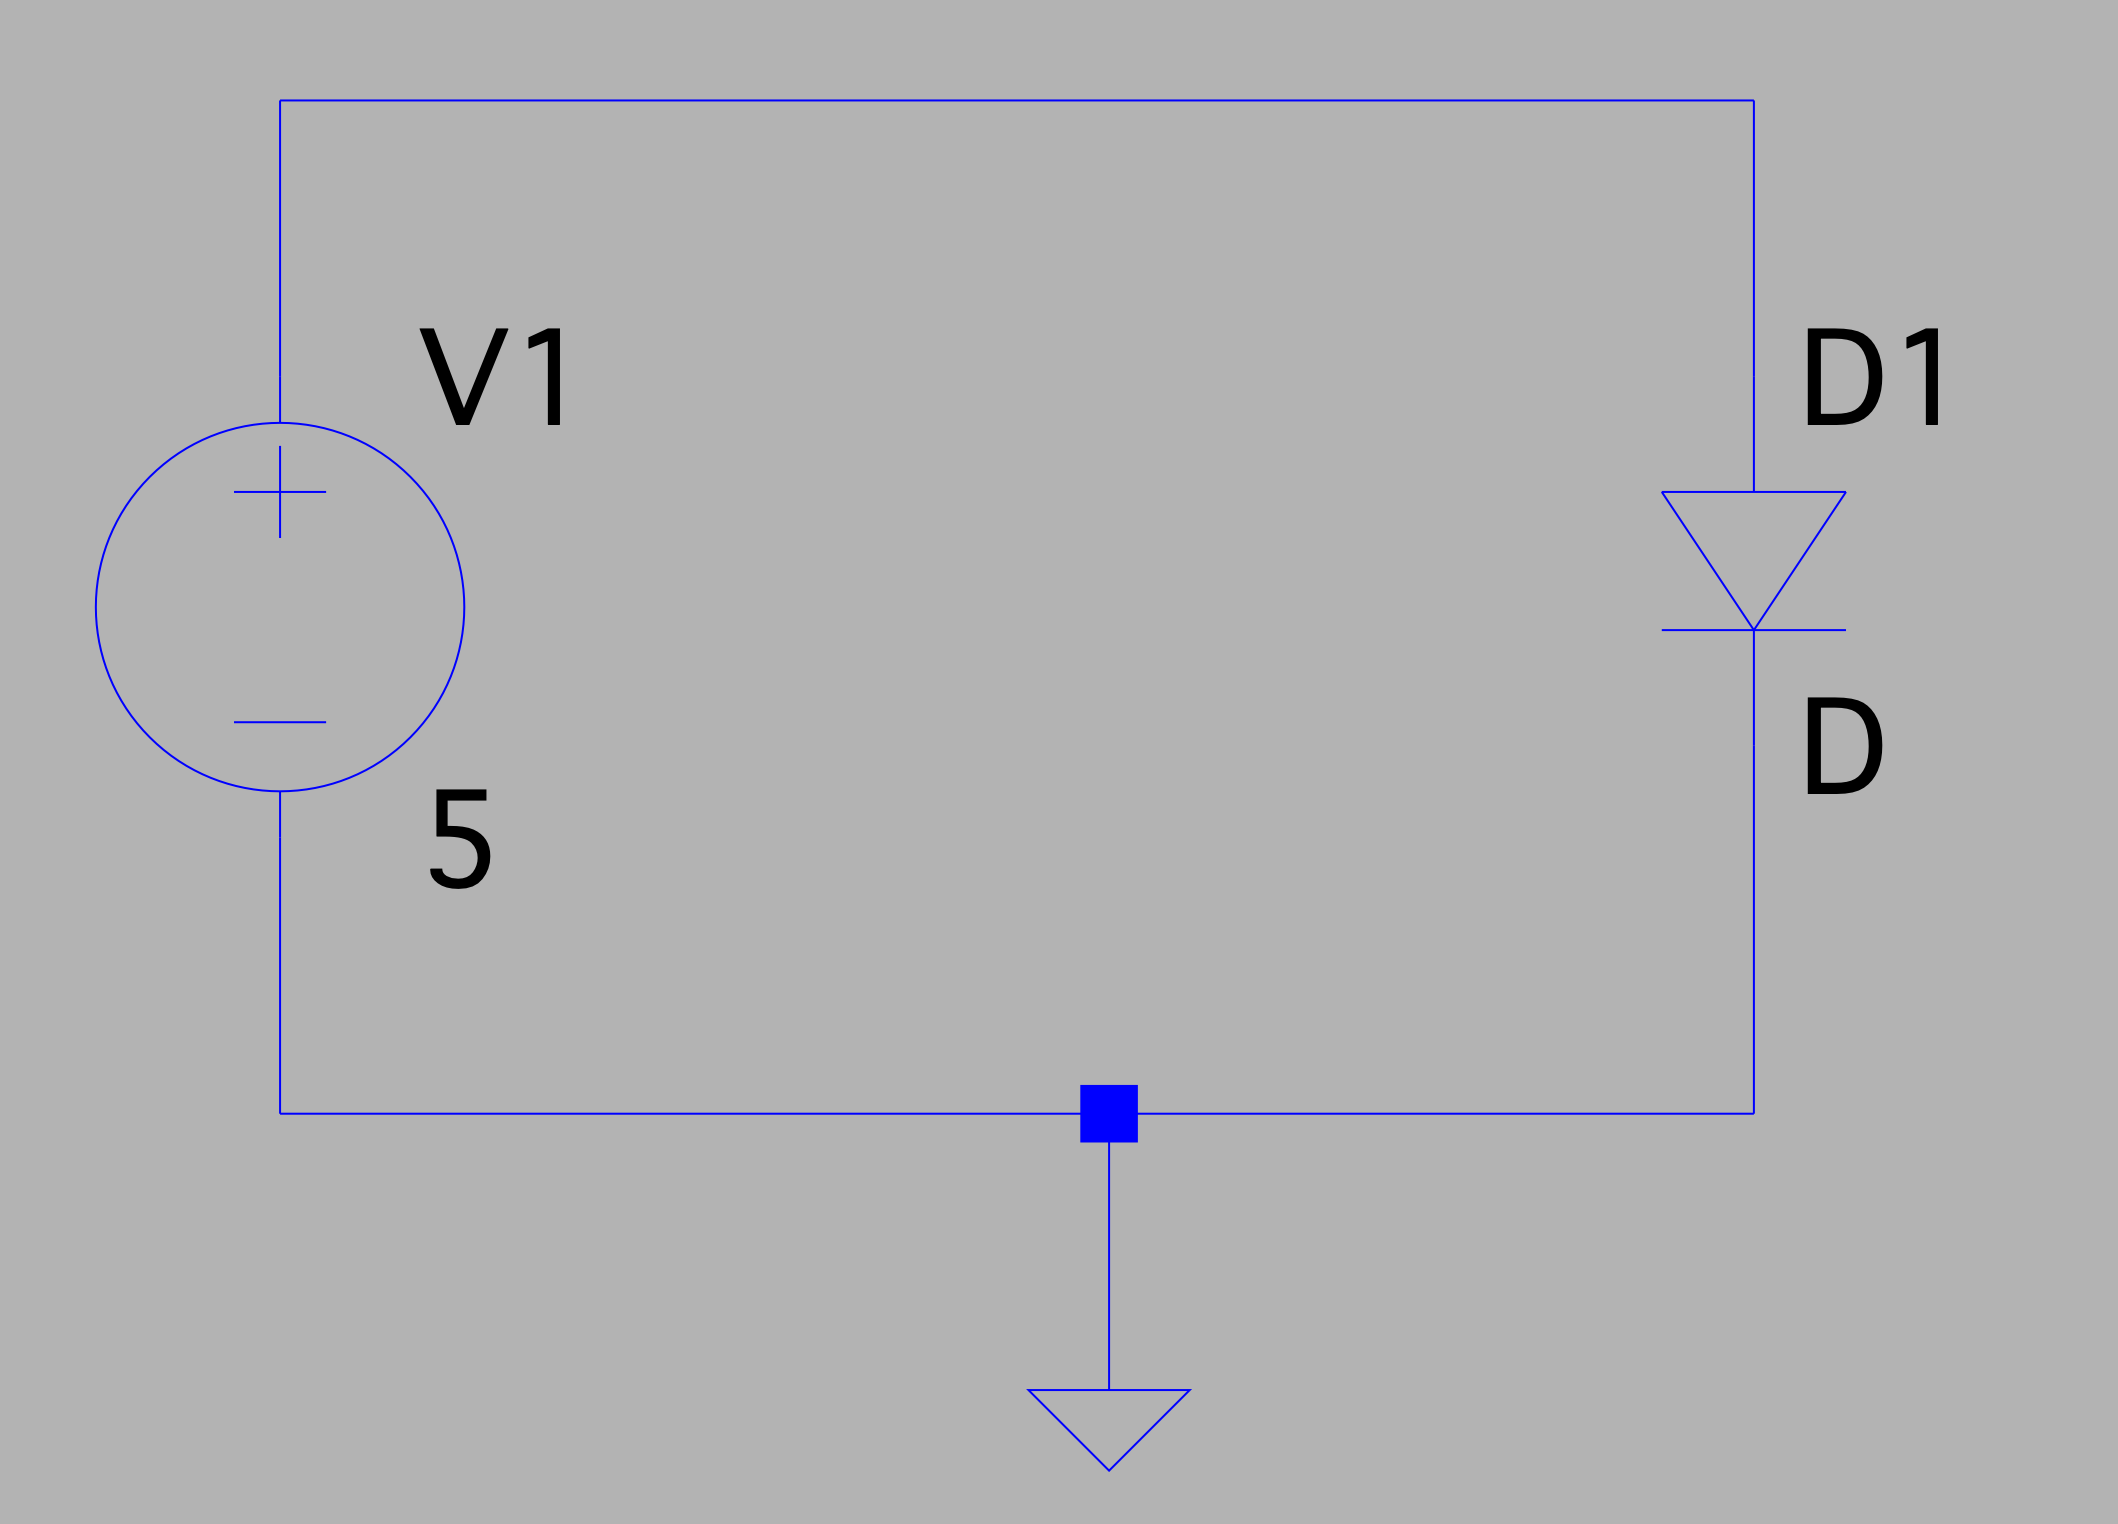
\includegraphics[width=\linewidth]{pictures/diode.png}
        \end{minipage} 
        & 
        \begin{minipage}{.7\textwidth}
        \begin{itemize}
          \item Speichert das Projekt direkt als neue Datei ab (File $->$ save as ) 
          \item Löscht den Wiederstand heraus (\textbf{F5}) 
          \item Öffnet erneut den Bauteileditor (\textbf{F2}) und für eine einfache Diode hinzu (sucht nach Diode \dots)
          \item Verdrahtet die Schaltung wieder vollstänndig (\textbf{F3})
        \end{itemize}
        \end{minipage} 
        \\
         & \\
         \hline
         \textbf{Konfiguration der Simulation} & \\
         \hline \\
         \begin{minipage}{.3\textwidth}
          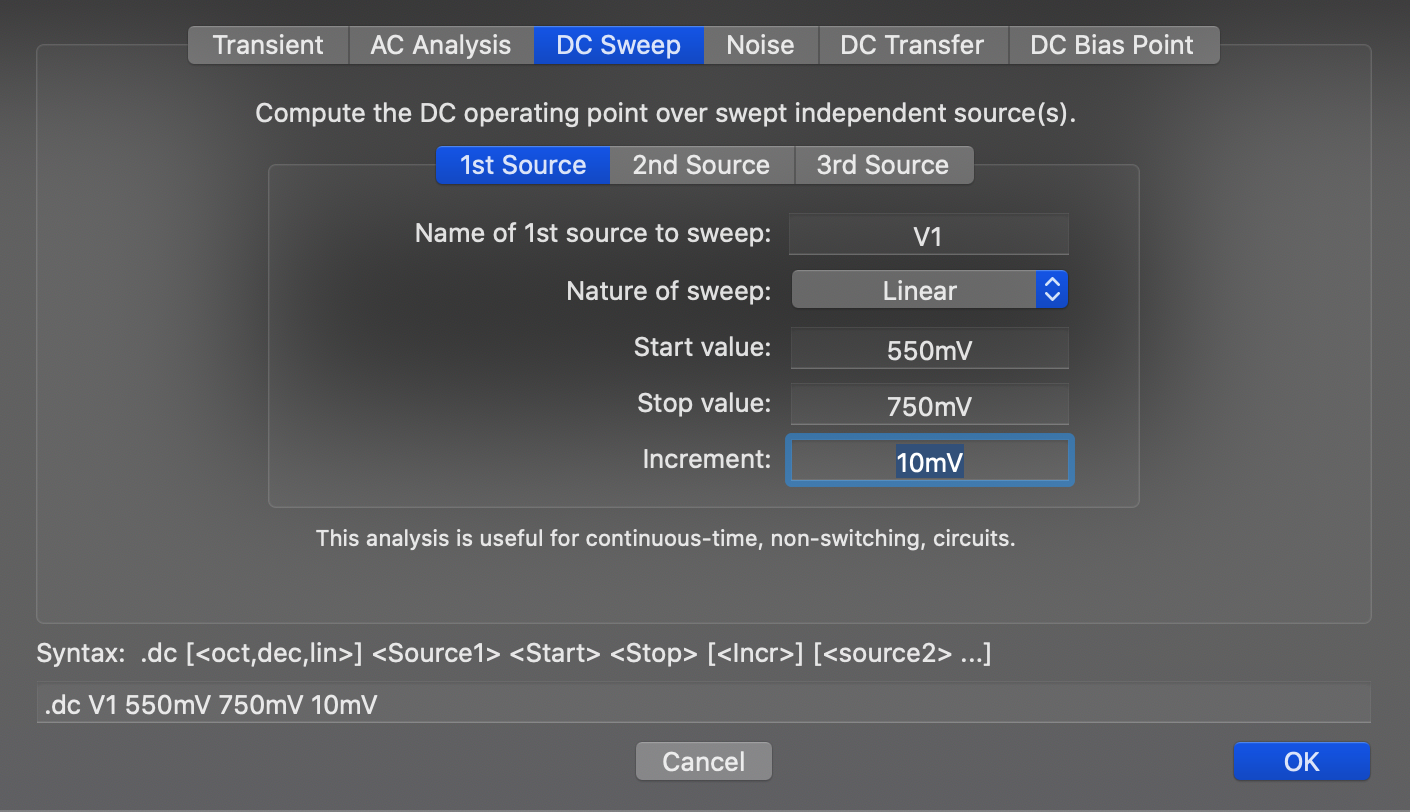
\includegraphics[width=\linewidth]{pictures/simulationcmd_2.png}
        \end{minipage} 
        & 
        \begin{minipage}{.7\textwidth}
        \begin{itemize}
          \item Im Menu Simulation, wählt \textbf{Edit simulation command} und bliebt beim DC Sweep. 
          \item Unser Ziel ist es den Stromverlauf durch die Diode zu messen. Dafür müssen wir die Spannung erhöhen. 
          Wir wissen, dass die notwendige Spannung im Bereich 600 - 700 mV liegen muss. 
          \item Daher konfigurieren wir die Spannungsquelle \textbf{V1} mit einem \textbf{linearen} Sweep von 550 bis 750 mV mit einer \textbf{Schrittweite} von 10 mV.
          \item Bestätigt mit \textit{OK} und fügt die Sumlationsansweisung dem schematic hinzu
        \end{itemize}
        \end{minipage} 
        \\
         & \\
         \hline
      \end{tabular}
    
    \end{table}
    
    \end{tiny} \end{spacing}
    
     \end{frame}
    
     \begin{frame}[t]{Diode}
    
      \begin{spacing}{0.9} \begin{tiny}
      \begin{table}[h!]
        \begin{tabular}{p{5cm} p{5cm}}
          \hline
          \textbf{Simulation und Analyse} & \\
          \hline \\
          \begin{minipage}{.5\textwidth}
            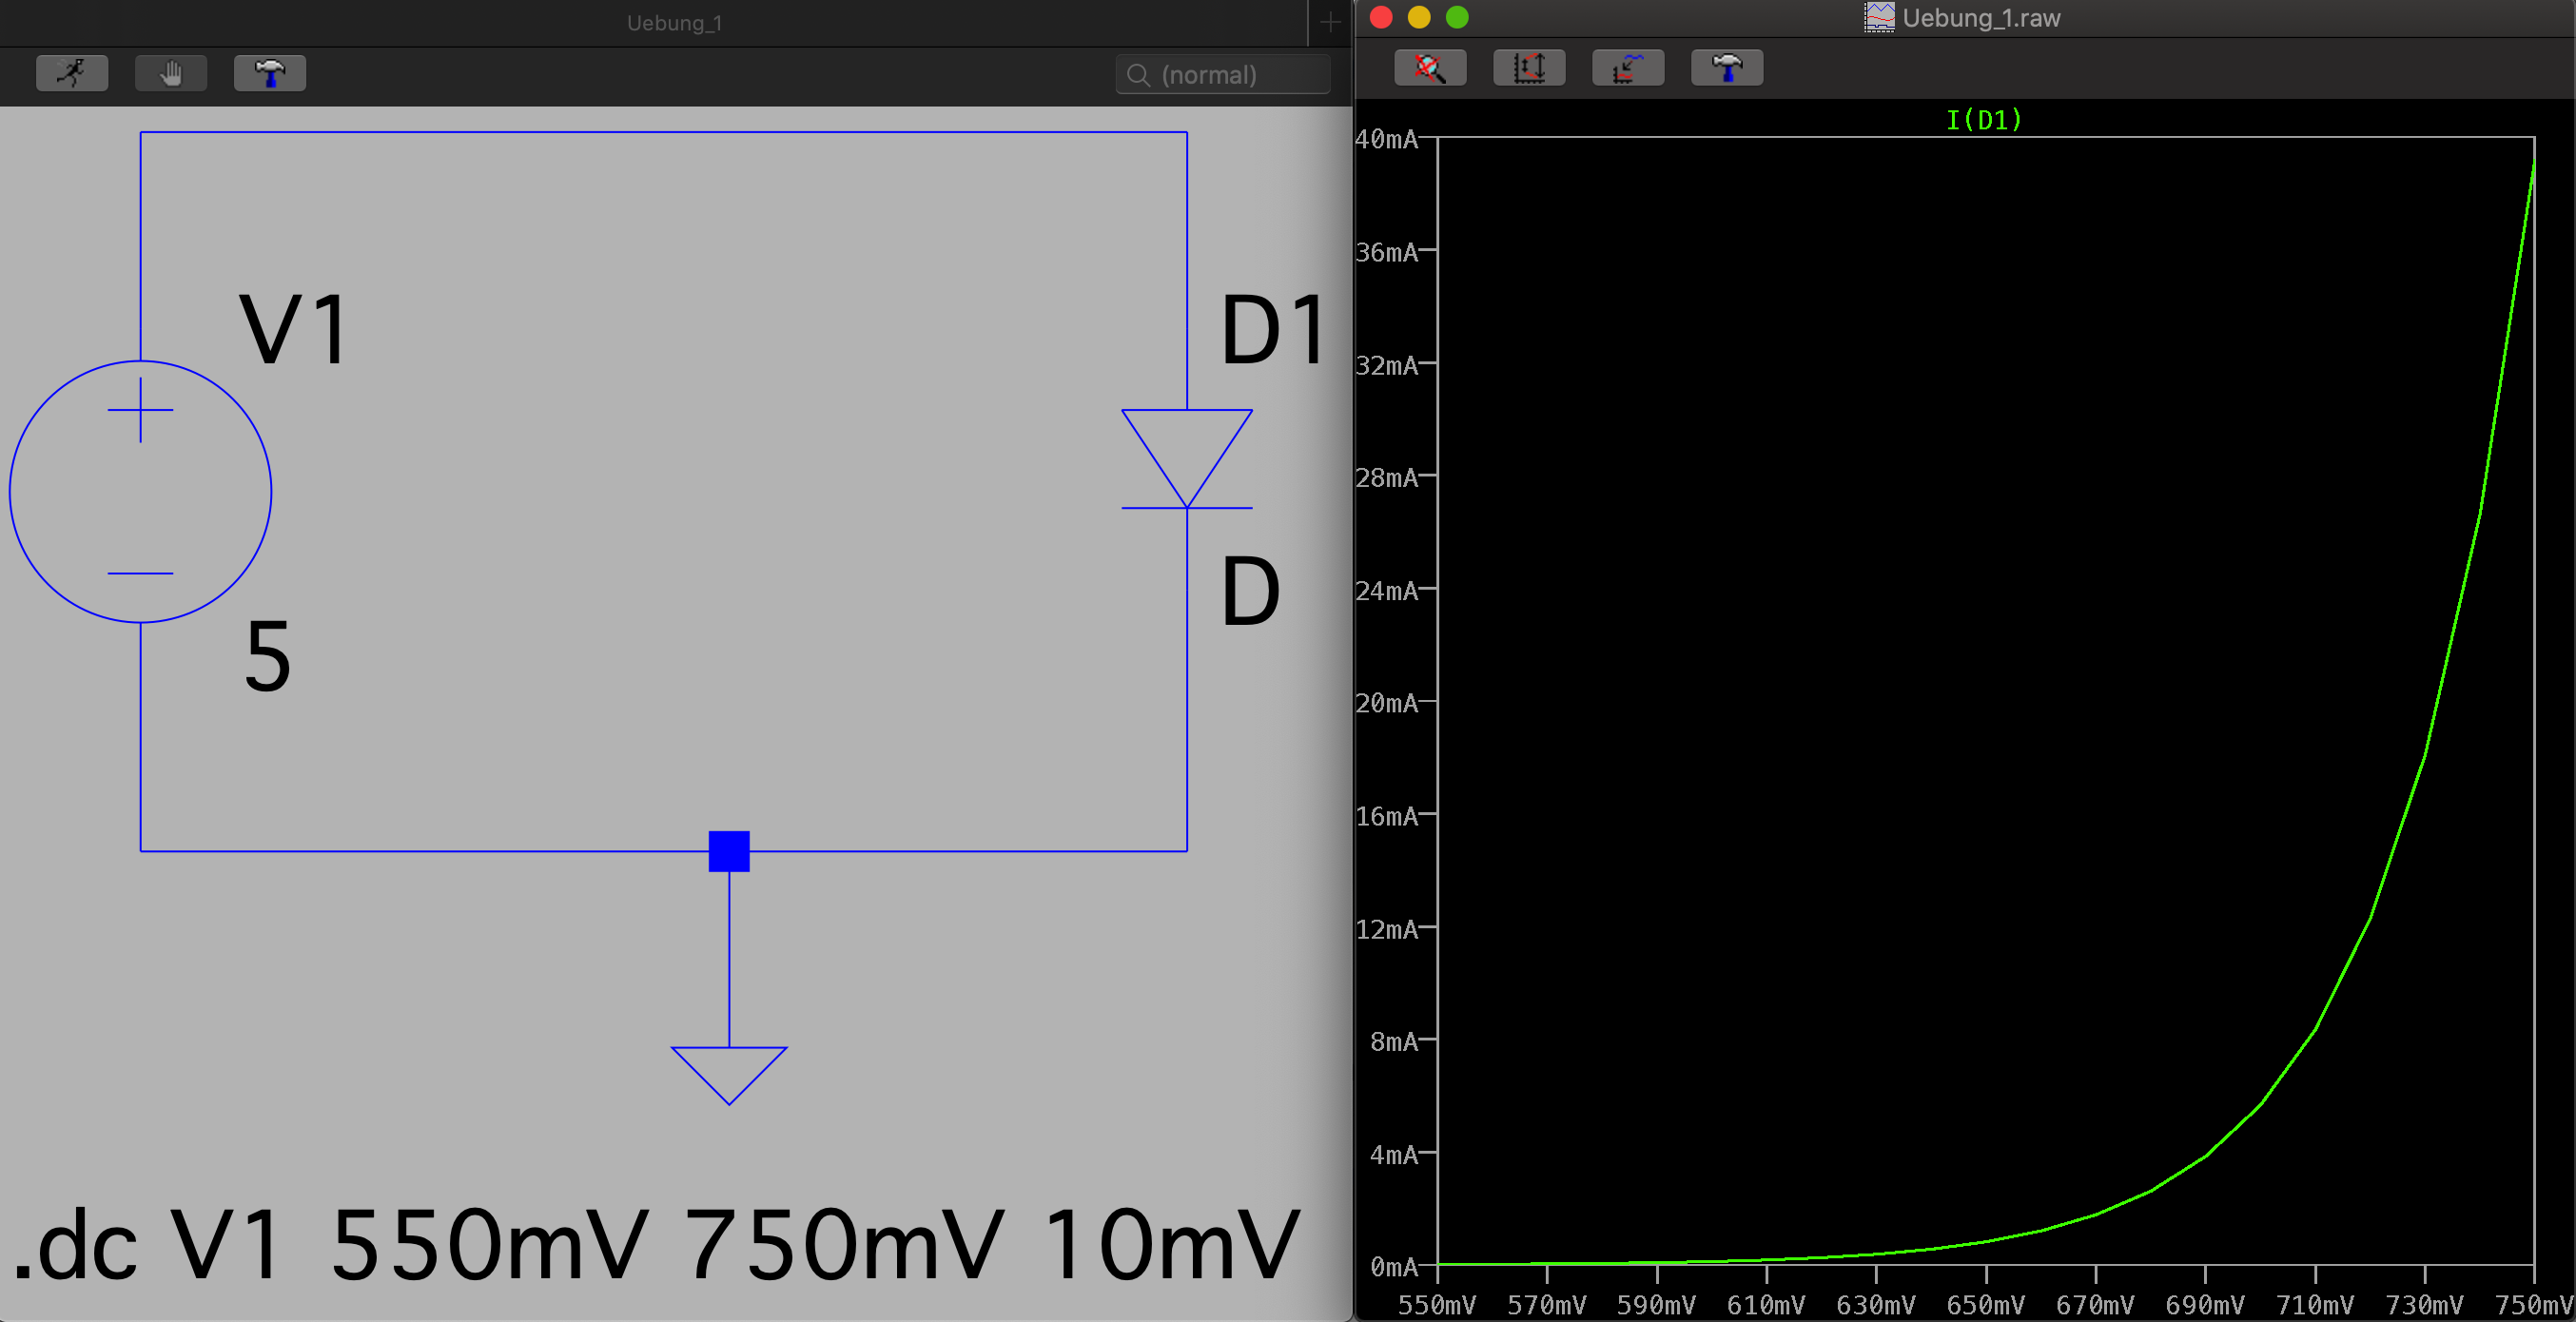
\includegraphics[width=\linewidth]{pictures/analysis_2.png}
          \end{minipage} 
          & 
          \begin{minipage}{.5\textwidth}
          \begin{itemize}
            \item Klickt auf 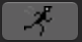
\includegraphics[scale=0.3]{pictures/run.png} (run) und LTSpice startet die Simulation
          \item Wir wählen \textbf{I(D1)}, den Strom durch die Diode.
          \end{itemize}
          \end{minipage} 
          \\
        \end{tabular}
      \end{table}
    \end{tiny} \end{spacing}
    
      \begin{spacing}{0.9} \begin{tiny}
        \begin{table}[h!]
          \begin{tabular}{p{10cm} }
            \hline
            \textbf{Ergebnis und Auswertung} \\
            \hline \\    
            Wie zu erwarten liefert dieses einfache Beispiel den Zusammenhang zwischen Strom, Spannung und Wiederstand. Probiert den Spannungsbereich des
            DC-Sweep von 550 - 750 mV auf 550 mV - 2V zu erhöhen.          
            \begin{itemize}
              \item Was fällt euch auf?
              \item Könnt ihr euch herleiten, warum man eine 
              Diode immer mit einem Vorwiederstand betreiben sollte? 
            \end{itemize}  
            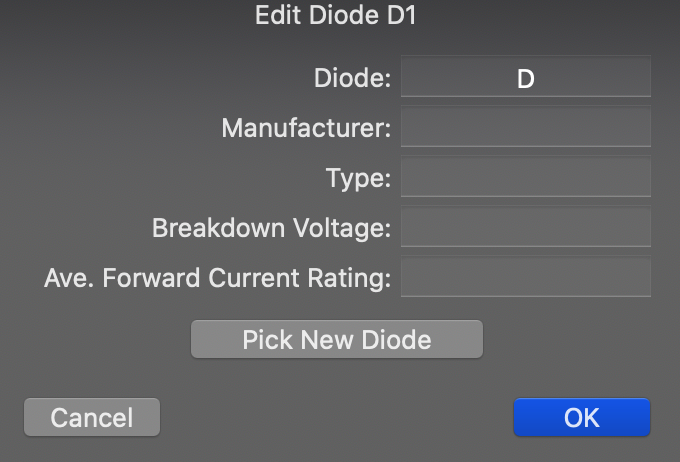
\includegraphics[scale=0.1]{pictures/diode_choice.png} \newline
            Mit einem rechten Mausklick auf die Diode könnte ihr die Dioden Typen variieren. (\textbf{pick new diode})
            Zum Beispiel von einer idealen aus dem obigen Beispiel zu einer beliebigen realen entsprechend dem Modell des Herstellers, schaut euch die Unterschiede an.
          \end{tabular}
        \end{table}
      \end{tiny} \end{spacing}
      
       \end{frame}